
\documentclass[]{article}
\usepackage[T1]{fontenc}
\usepackage[utf8]{inputenc}
\usepackage{color}
\usepackage{hyperref}
\usepackage{float}
\usepackage{datetime}
\usepackage{graphicx}
\usepackage{amsmath}
\usepackage{attachfile}
\usepackage[margin=3cm]{geometry}
\graphicspath{{./assets}}
\hypersetup{
	colorlinks=true,
	linktoc=all,
	linkcolor=black,
}

\title{Analysis of natural language complexity used by open-source developers\\ \large Introduction to Natural Language Processing}
\author{Komlichenko Ilya, Krzemiński Piotr, Monicz Kamil, \\Piotrowska Weronika, Wojnarowski Marcin}
\date{\monthname, \the\year}
	
\newcommand{\secref}[1]{{(Section \hypersetup{linkcolor=blue}\ref{#1})}}

\newcommand{\figref}[1]{{(Fig. \hypersetup{linkcolor=blue}\ref{#1})}}

\begin{document}

\maketitle

\tableofcontents
\newpage


\section{Motivation}

In order to improve our NLP skills, we are going to complete simple natural language analysis. The topic of choice should be close to our hearts so we stay engaged throughout the project. In addition, the source data should be freely accessible, so it is easy to work with. And so, our analysis will focus on the natural language complexity used by developers of various programming languages who contribute to open-source platforms (such as GitHub).

We hypothesize that language with a lower barrier of entry (such as Python) will exhibit a lower natural language complexity than languages that expect a higher level of expertise (such as C). Additionally, we are aware of different demographics of programming languages thus expect scientific/research focused languages (such as Julia) programmers will naturally use a more complex natural language to express ideas/problems.

\section{Data sourcing}

The linguistic data will be primarily scraped from the GitHub issues, where developers, using natural language, often describe bugs or feature requests related to some piece of software. And since the code there is publicly available, it is easy to assign a specific programming language to it.

\subsection{Text processing}

Every issue will be assigned a complexity/readability score based on industry-standard algorithms and bucketed into their respective programming language. For example, one could compute Flesch-Kincaid Grade Level or check the frequency of passive sentences.

\subsection{Scraping procedure}

Using the official GitHub API we will first look through active GitHub users and then issues posted by the given user. Only issues written in English will be considered, where the language detection can be trivially and effectively done with simple methods such as letter frequency distribution comparison. The most popular programming language used by a given programmer (as determined by GitHub) will determine the said language label assigned to the scraped issue. We cannot go with the programming language used in the repository where the issue was posted due to the simple fact that code of a non-library repository is usually not used directly by a issue poster, thus being a false connection between the content of an issue and a programming language used by the poster.

Data scraped from GitHub will be cleaned up by removal of any non-natural language texts such as code blocks. We suspect that the dataset will be still full of true-negatives and will require manual labor to review our samples. Finally, the dataset will simply consist of two dimensions: text (issue content) and a label (programming language).

We want to focus on a specific subset of languages with a fairly balanced distribution between classes, also taking into account the repetition of issue posters.

\section{Functionalities}

After scrapping the data, we are planning to perform following operations in order to give us a more complete insight

\begin{enumerate}
	\item Basic text analysis -- this includes average length of sentences, average length of words, most common word occurring etc. We are expecting developers of more complex programming languages to use more sophisticated language in the reported issues, this includes less grammar mistakes, longer sentences and words.

	\item Frequency of passive sentences -- in order to identify passive sentences we will use Part Of Speech tagging (POS). In English, a passive sentence can be defined by the place of the verb in the sentence and the form of this verb. We suspect the data to have high frequency of passive sentences, as it describes development issues.

	\item Flesh-Kincaid Grade Level -- by evaluating the Flesh-Kincaid grade level, we can determine whether the text is readable to an average, non-developer person. It measures the length of the sentences and syllables per words, which indicated the easy to read or not. We expect developers of more complex programming languages to write harder to read issue descriptions.

	      \[0.39\left(\frac{\text{total words}}{\text{total sentences}}\right) + 11.8\left(\frac{\text{total syllables}}{\text{total words}}\right) - 15.59\]

	\item Flesh redability score -- similarly to Flesh-Kincaid Grade Level, this score is used to measure level of difficulty when reading a text. We compute the score as follows:

	      \[206.835 - 1.015\left(\frac{\text{total words}}{\text{total sentences}}\right) - 84.6\left(\frac{\text{total syllables}}{\text{total words}}\right)\]
\end{enumerate}

We hope that after obtaining this data, there will be interesting conclusions that there exists dependency between a developer's primary programming language and the natural language he or she uses when describing issues on GitHub.

\section{Results}
\subsection{Basic text analysis}
\begin{enumerate}
    \item Average text length
    
    This graph presents average length of an issue description. We can observe that this value is similar for every analyzed language.
    
    
    \begin{figure}[H]
    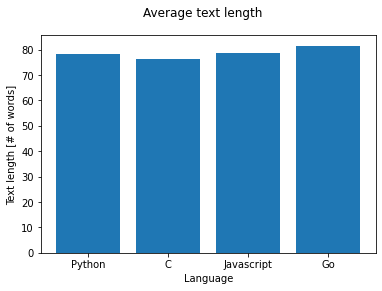
\includegraphics[width=8cm]{resources/avg_len.png}
    \centering
    \end{figure}
    
    \item Average lexical diversity of a single issue
    
    This value is the average lexical diversity of a single issue. This value is obtained by dividing the set of tokens over the number of words in a single issue. The value is then averaged for each language. We can observe that this issue is similar among every language.
    
        \begin{figure}[H]
    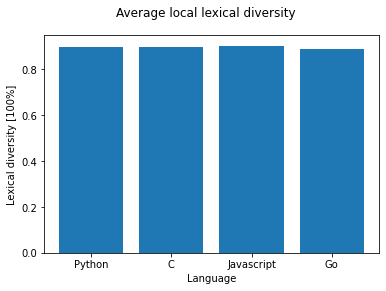
\includegraphics[width=8cm]{resources/lex_div_single.png}
    \centering
    \end{figure}
    
    \item Total lexical diversity
    
    This value is the lexical diversity of all issues among the language. It is obtained by dividing set of tokens over number of all words in all issues. We can see that the lexical diversity is small for every language, which means all of the programmers write similar issue descriptions. However, C programmers tend to use the most diverse descriptions.
    
            \begin{figure}[H]
    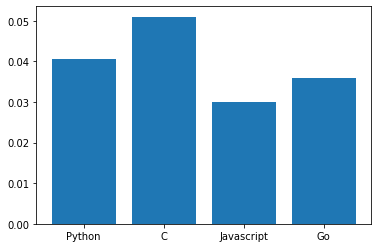
\includegraphics[width=8cm]{resources/lex_div_total.png}
    \centering
    \end{figure}
    
    \item Average word length
    
    This is the average word length for every language. We can observe that this value is similar among all languages.
    
                \begin{figure}[H]
    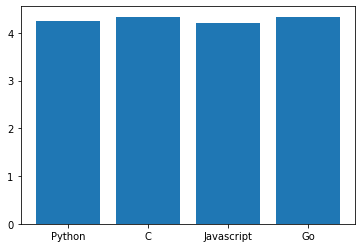
\includegraphics[width=8cm]{resources/word_len.png}
    \centering
    \end{figure}
    
    \item Percentage of words over 10 characters
    
    Here is the percentage of words over 10 characters used in all issue descriptions among all languages. We can observe that all the programmers use long words with similar frequency.
    
                    \begin{figure}[H]
    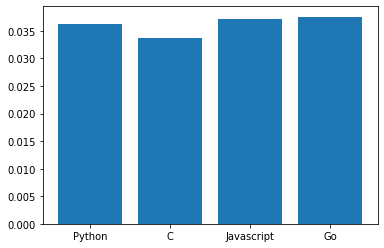
\includegraphics[width=8cm]{resources/long_words.png}
    \centering
    \end{figure}
    
\end{enumerate}

\subsection{Frequency distributions}
In this section, we present the frequency distribution of tokens in the text. We can see the most common words used, as well as the cumulative value of this words. 

\begin{enumerate}

\item Python

In Python, the most commod words are would, like, code, use and using. Given over 2 900 000 tokens in the text, top 20 words make up to 37\% of the whole data.

                        \begin{figure}[H]
    \includegraphics[width=8cm]{resources/freq_Python.png}
    \centering
    \end{figure}
    
    \item C
    
    In C language, the most common words used are would, file, like, use and code. We can see that, given over 2 600 000 tokens in the text, top 20 words made up to 34\% of the total text. 
    
                        \begin{figure}[H]
    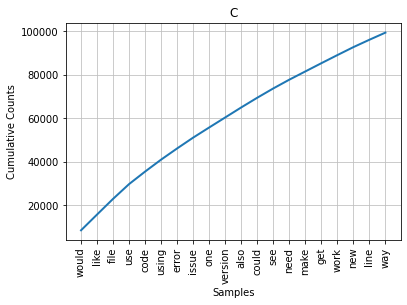
\includegraphics[width=8cm]{resources/freq_C.png}
    \centering
    \end{figure}
    
    \item JavaScript
    
    In JavaScript, the most common words are would, like, use, using, could. Given 3 700 000 tokens in the whole text, top 20 words make up to over 40\% of the whole data.
    
                            \begin{figure}[H]
    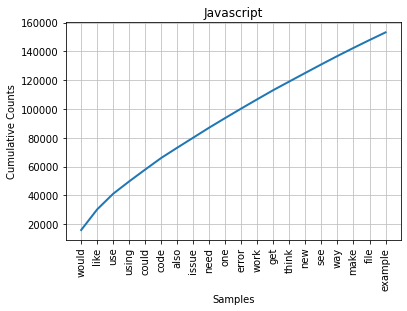
\includegraphics[width=8cm]{resources/freq_java.png}
    \centering
    \end{figure}
    
    \item Golang
    
    In Go, most common words are would, like, go, use, using. Given over 4 500 000 tokens, the top 20 make up to 40\% of the whole text.
    
                                \begin{figure}[H]
    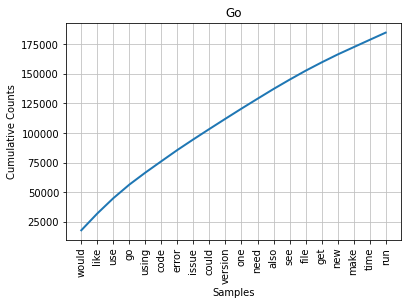
\includegraphics[width=8cm]{resources/freq_Go.png}
    \centering
    \end{figure}
    
    
\end{enumerate}

We can observe that among all languages, issue comments contain variations of words would and use. The most informative feature is that C programmers use word 'file' a lot, probably to low-level file access provided by C. Golang programmers use word 'go' a lot, which may come from the language name.

\subsection{Frequency of passive sentences}

As expected, the frequency of passive sentences is high for all languages (in comparison to 10\% in most books), as it describes specific bugs in the code. One can see that C programmers use passive sentences the most, achieving almost 40\% of total passive sentences.

                                \begin{figure}[H]
    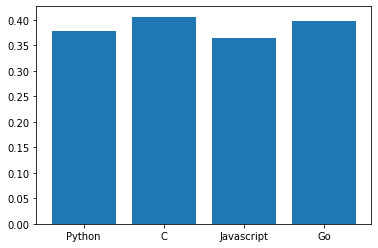
\includegraphics[width=8cm]{resources/passives.png}
    \centering
    \end{figure}
    
\subsection{Flesch readability score}

We can see that all of the languages fall into 60-70 interval, which leads them to be classified as easily understood by 13- to 15-year-old students. This score takes into account number of syllables per word and sentence length, which, as established earlier, was not high in most cases.

    \begin{figure}[H]
    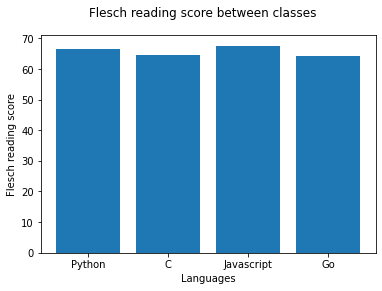
\includegraphics[width=8cm]{resources/flesch.png}
    \centering
    \end{figure}
    
\subsection{Flesch-Kincaid grade level}

In this case, all languages scored below 10, which makes them extremely difficult to read, understood only by university graduates. However this metric also takes into account number of words and syllables per sentence, it is much different than the previous Flesch metric. However, in most cases any text has higher Flesch reading score than Flesch-Kincaid grade level. 

    \begin{figure}[H]
    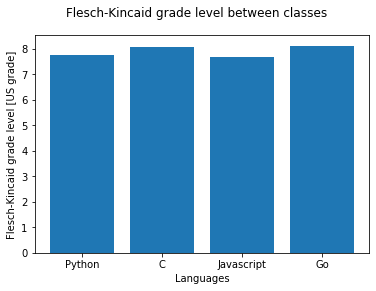
\includegraphics[width=8cm]{resources/flesh_kincaid.png}
    \centering
    \end{figure}

% \section{Attachments}

% \begin{enumerate}
% \item \textattachfile[color=0 0 1]{file}{file} -- Description
% \end{enumerate}


\end{document}
